\chapter{Self-Consistent Fields}
\section{Massless Klein-Gordon Field with Dirichlet boundary conditions}

\begin{figure} \centering 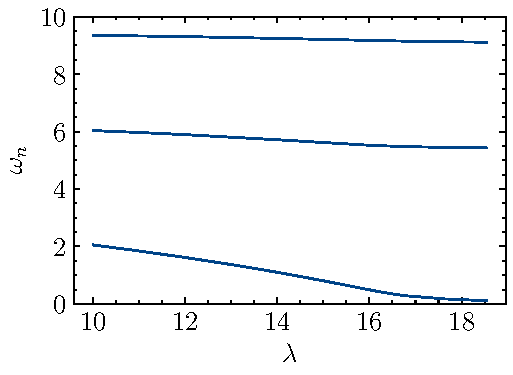
\includegraphics[width=0.8\linewidth]{figures/dirichlet/eigenvaluesHadamardDirichlet.pdf} \caption{Energy of the first three positive energy modes of the massless, charged Klein-Gordon field with Dirichlet boundary conditions as a function of the background electric field strength $\lambda$. The orange curves represent the energies in the external field approximation, where the critical value $\lambda_c$ emerges. The blue curves correspond to the self-consistent solutions of the Klein-Gordon-Maxwell equations with Dirichlet boundary conditions for the scalar field $\phi$.  The bottom curves correspond to $\omega_1$, the middle curves to $\omega_2$ and the top curves to $\omega_3$.} \label{fig:eigenvaluesHadamardDirichlet} \end{figure}

In this section, we present the results of the self-consistent solutions to the Klein-Gordon-Maxwell equations, with Dirichlet boundary conditions for the charged massless Klein-Gordon field $\phi$ using the procedure outlined in the previous chapter.

Figure \ref{fig:eigenvaluesHadamardDirichlet} shows the energy of the first three modes of the $\phi$  field as a function of the increasing background electric field strength $\lambda$. In blue, for the self-consistent $\phi$  and for reference, the external field approximation, in orange.

The lower curves correspond to the energy $\omega_1$ of the fundamental mode, the middle curves to $\omega_2$ and the upper curves to $\omega_3$.
The orange $\omega_1$ curve shows the appearance of the critical $\lambda_c$, i.e. the electric field strength for which the energy $\omega_1$ of the fundamental mode goes to zero. 
Figure \ref{fig:eigenvaluesHadamardDirichlet} shows a very similar low-$\lambda$ behavior between the self-consistent solutions and the external field approximation. It is however in the high-$\lambda$ regime where the relevance of the back-reaction of the Klein-Gordon field appears.
Indeed, as the strength of the external electric field increases, the charged $\phi$ screens the external charges, thus raising the energy of the field and avoiding the instabilities that the external field approximation presents.

Due to unsolved \note{As of the twenti-fifth of February} technical issues, the full $\lambda$-parameter space cannot be sampled, disabling us to definitely say that for any $\lambda$ the back-reaction of $\phi$ is able to stabilize the self-consistent solutions.

\begin{figure} \begin{subfigure}{0.5\textwidth} \centering
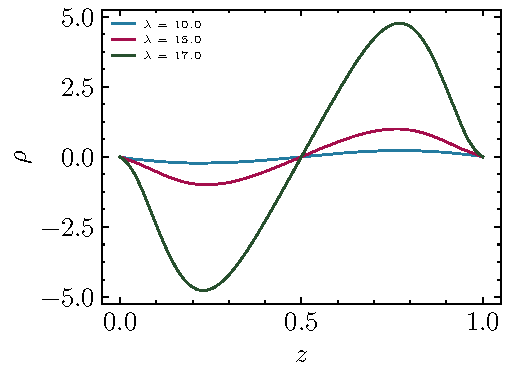
\includegraphics[width=1\linewidth]{figures/dirichlet/vacuumPolarizationEvolution.pdf}
\label{fig:HadamardVacuumPolarization1}
\end{subfigure}
\hfill
\begin{subfigure}{0.5\textwidth} 
\centering
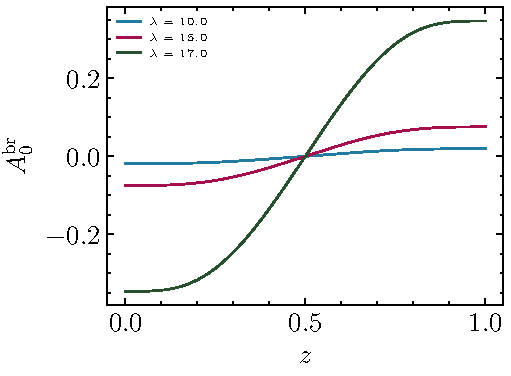
\includegraphics[width=1\linewidth]{figures/dirichlet/A0InducedEvolution.pdf} 
\label{fig:HadamardVacuumPolarization2} 
\end{subfigure}
\caption{Self-consistent vacuum polarization of the massless Klein-Gordon field $\rho(z)$ (left) and their corresponding induced potential $A_0^\text{br}(z)$ (right) for selected values of $\lambda$, as indicated in the legend. } \label{fig:HadamardVacuumPolarization} \end{figure}

Figure \ref{fig:HadamardVacuumPolarization} illustrates both the self-consistent vacuum polarization $\rho(z)$ and the electrostatic potential $A_0^\text{br}(z) = -\int_{\frac{1}{2}}^z dz' \int_0^{z'}dz''{\rho}(z'')$ for selected values of $\lambda$. The back-reaction grows rapidly with $\lambda$ for higher values of $\lambda$. 
To better visualize the dependence of the vacuum polarization on $\lambda$, we study the induced charge resulting from the background electric field. The boundary conditions imposed in the equation \eqref{eq:boundary-conditions-A0} imply that the induced charge 
$$Q_{\text{total}} = \int_0^1 \rho(z) dz = 0.$$
It is easy to check that this holds since $\rho(z) = -\rho(1-z)$.

Instead, we focus on the induced charge in the left half of the $z$-region:
$$Q_{I} = \int_0^\frac{1}{2} \rho(z) dz.$$
In one spatial dimension, $Q_I$ corresponds with the value of the induced electric field at $z=\frac{1}{2}$. We use this as a measure of the strength of the back-reaction. This induced charge effectively screens the background electric field, so the measured electric field at $z=\frac{1}{2}$ is $Q_I + \lambda$. 


\begin{figure}
\begin{subfigure}{0.5\textwidth}
    \centering
    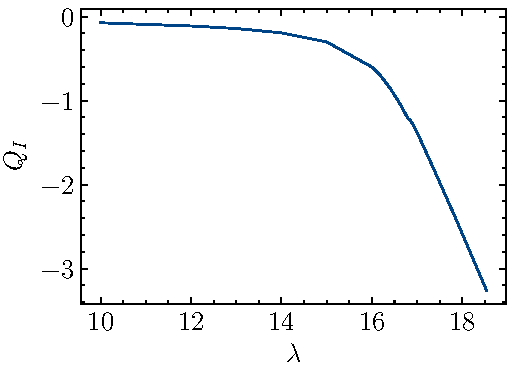
\includegraphics[width=0.95\linewidth]{figures/dirichlet/inducedCharge.pdf}
\end{subfigure}
\begin{subfigure}{0.5\textwidth}
    \centering
    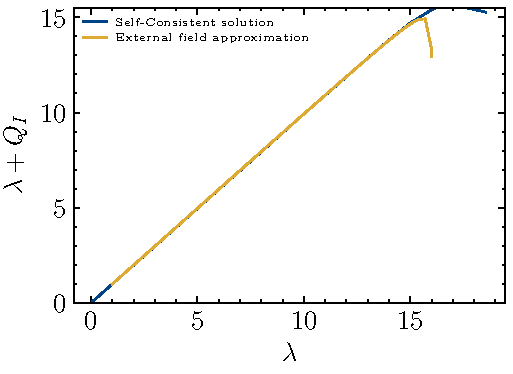
\includegraphics[width=0.95\linewidth]{figures/dirichlet/electricFieldInduced.pdf}
\end{subfigure}
 \caption{The induced electric charge $Q_I = \int_0^{1/2}\rho(z)dz$ in the region $z\in[0,1/2]$ as a function of $\lambda$ (left pane) and the total electric field $\lambda + Q_I$ at the mid-point as a function of $\lambda$ (right pane). In orange, the results for the external field approximation (i.e. no inclusion of the back-reaction of the Klein-Gordon field), in blue the results for the self-consistent solution. }
\label{fig:induced-charge}
\end{figure}


Figure \ref{fig:induced-charge} shows the induced charge $Q_I$  as a function of $\lambda$ (left panel), and the screened total charge $\lambda + Q_I$ observed at $z=\frac{1}{2}$ (right panel). 
These quantities are again displayed both for the self-consistent $\phi$ (blue) and, for reference, the external field approximation (blue).

This figure illustrates two distinct behaviors of the self-consistent $\phi$ as $\lambda$ increases. For low $\lambda$ ($\lambda \ll \lambda_c$) the strength of the polarization\textemdash  measured here using the induced charge $Q_I$\textemdash exhibits a linear dependence on $\lambda$.
However, once $\lambda$ approaches and surpasses the critical threshold $\lambda_c$, the self-consistent solution deviates significantly from the external field approximation. The back-reaction screens the external charges, mitigating the divergence of the vacuum polarization. As a result, the total electric field at $z=1/2$, given by $\lambda + Q_I$ (as seen in the right panel of Figure \ref{fig:induced-charge}), remains under $\lambda_c$. More importantly, this screening mechanism ensures $\abs{Q_I} < \lambda$, which is unphysical. 
%Figure \ref{fig:firstModeRho} illustrates the contributions of the modes $n=\pm1$ to the total charge density. In the top panel, the charge density $\rho_{1}$ associated to $n=1$, in the middle panel the charge density $\rho_{-1}$ associated to $n=-1$, and in the bottom panel their total contribution to the total charge density $\rho_1 + \rho_{-1}$. Notice how $\rho_1$ behaves as one would expect a positively charged particle to behave under a right-pointing electric field. Also notice how for a certain value of $\lambda$, a region of negative charge appears. Since $$\rho_n = (\omega_n + \lambda(z-1/2) - \epsilon A_0^\text{br}) \lvert\phi_n\rvert^2$$, this region corresponds to $$ $$

%\begin{figure}
%    \centering
%    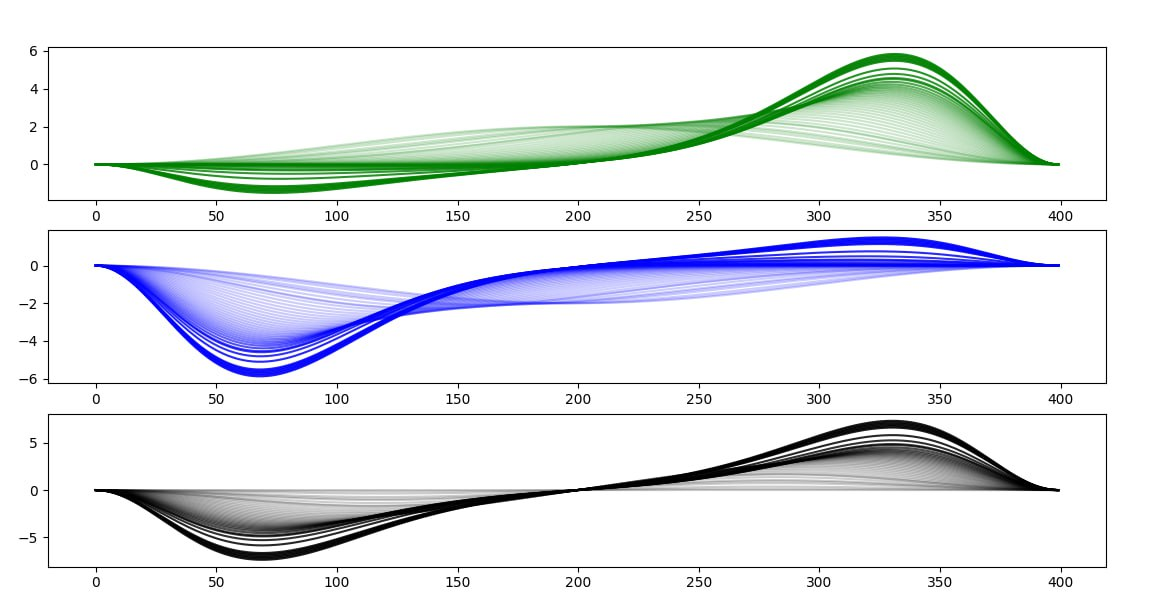
\includegraphics[width=0.75\linewidth]{figures/dirichlet/firstModeRho.jpg}
%    \caption{The charge density associated with the modes $n=1$ (top panel), $n=-1$ (middle panel) and their contribution to the total vacuum polarization $\rho_{1} + \rho_{-1}$ (bottom panel) for increasing $\lambda$ values, with dimmer curves corresponding to lower $\lambda$ values, and opaque curves corresponding to higher $\lambda$. }
%    \label{fig:firstModeRho}
%\end{figure}

%%%%%%%%%%%%%%%%%%%%%%%%%%%%%%%%%%%%%%%%%%%%%%%%%%%%%%%%%%%%

\subsection{Massive Klein-Gordon field with Dirichlet boundary conditions}

\begin{figure}
\begin{subfigure}{0.5\textwidth}
    \centering
    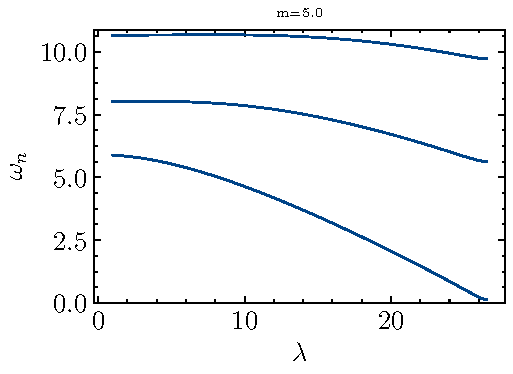
\includegraphics[width=\linewidth]{figures/dirichlet/eigenvaluesDirichlet m5.pdf}
\end{subfigure}    
\begin{subfigure}{0.5\textwidth}
    \centering
    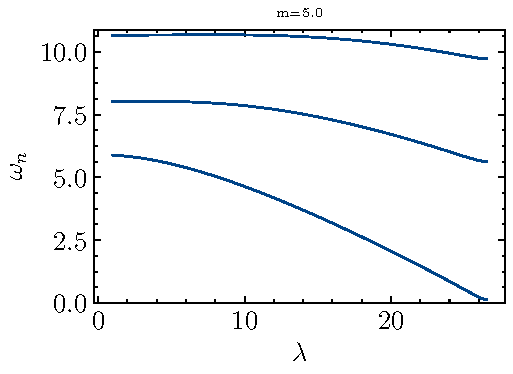
\includegraphics[width=\linewidth]{figures/dirichlet/eigenvaluesDirichlet m5.pdf}
\end{subfigure}    
\caption{The energy of the first three modes of the massive self-consistent Klein-Gordon field for the masses $m=5$ (left panel), $m=10$ (right panel).\note{the m=10 case is under construction}}
    \label{fig:eigenvaluesHadamardDirichletMassive}
\end{figure}

Following the same structure as in the previous section, this subsection presents the results for the self-consistent massive Klein-Gordon field with Dirichlet boundary conditions.  Figure \ref{fig:eigenvaluesHadamardDirichletMassive} presents the energies of the first three modes $\omega_1, \omega_2, \omega_3$ of $\phi$ resp. in the lower, middle, and upper curves, for increasing values of $\lambda$.

 \begin{figure}
\begin{subfigure}{0.5\textwidth}
     \centering
     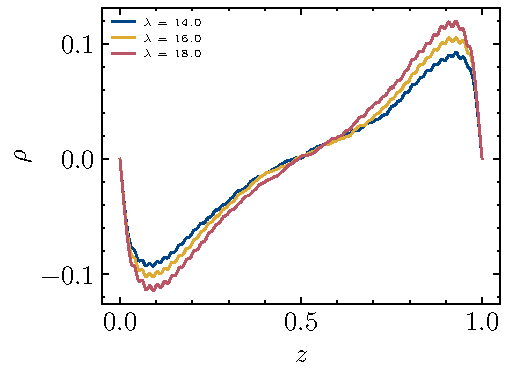
\includegraphics[width=\linewidth]{figures/dirichlet/vacuumPolarizationEvolution_M_5.pdf}
\end{subfigure}     
\begin{subfigure}{0.5\textwidth}
     \centering
     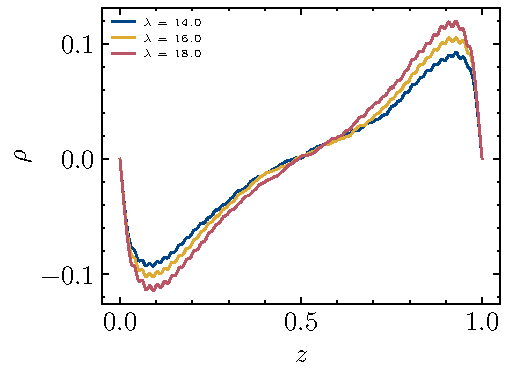
\includegraphics[width=\linewidth]{figures/dirichlet/vacuumPolarizationEvolution_M_5.pdf}
\end{subfigure}     
\caption{The vacuum polarization of the self-consistent massive Klein-Gordon field for the masses $m=5.0$ (left panel) and $m=10.0$, right panel, and for selected $\lambda$ values, pointed out in the legend.}
     \label{fig:vacuum-polarization-massive-dirichlet}
 \end{figure}

Additionally, Figure \ref{fig:vacuum-polarization-massive-dirichlet} presents the self-consistent vacuum polarization of the massive Klein-Gordon field for two different mass values: $m=5$ (left panel) and $m=10$ (right panel). 

 We observe that, in the massive case, the vacuum polarization is more strongly localized near the boundaries compared to the massless case.
 This effect arises  because more massive fields present a shorter Compton wavelength $\bar{\lambda} = 1/m$ (not to be confused with the background electric field strength), which  determines the characteristic scale of the fluctuations of the field.
%%%%%%%%%%%%%%%%%%%%%%%%%%%%%%%%%%%%%%%%%%%%%%%%%%
\section{Massive Klein-Gordon field with Neumann boundary conditions}

This section reports the self-consistent solutions of the Klein-Gordon-Maxwell equations when considering Neumann (attractive) boundary conditions. Figure \ref{fig:neumann-eigenvalues evolution.} shows the energy of the first three modes\footnote{Note the apparition of the $\phi_{0+}$ mode and its associated $\omega_{0+}$ energy when considering Neumann boundary conditions.} of the Klein-Gordon field as $\lambda$ increases. Following a similar notation as Figure \ref{fig:eigenvaluesHadamardDirichlet} the bottom curve corresponds to the energy $\omega_{0+}$ of the zeroth mode, the middle curve to the $\omega_1$ energy of the first mode, and the top curve $\omega_2$ of the second mode. We observe a slight increase of the energy of $\omega_1$ as $\lambda$ increases, but the overall behavior of the energy stays similar to the Dirichlet boundary conditions case.

The lowest energy of the Klein-Gordon field, $\omega_{0+}$ (in the case of Neumann boundary conditions), behaves similarly to the  energy $\omega_1$ observed in Figure \ref{fig:eigenvaluesHadamardDirichlet} from the previous section.  As $\lambda$ increases we observe a decrease in the energy, which slows down as the back-reaction of the Klein-Gordon field grows more pronounced.

\begin{figure}
    \centering
    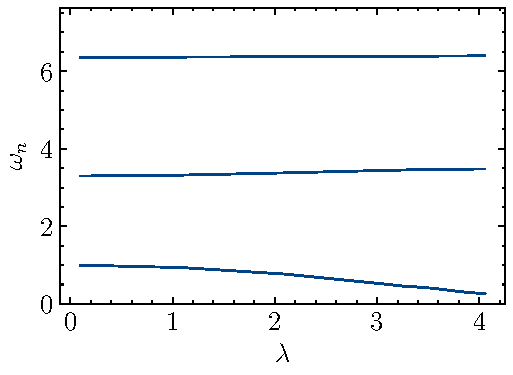
\includegraphics[width=0.75\linewidth]{figures/neumann/eigenvalues.pdf}
    \caption{The first three energies of the massive ($m=1$) Klein-Gordon field with Neumann boundary conditions. The bottom line corresponds to the $\omega_{0+}$ mode, the middle line to the $\omega_1$ and the top line to $\omega_2$.}
    \label{fig:neumann-eigenvalues evolution.}
\end{figure}

Figure \ref{fig:vacuumPolarizatoinEvolutionNeumann} shows the self-consistent vacuum polarizations $\rho$ and induced electric potentials $A_0^\text{br}$ for selected values of $\lambda$, as indicated in the legend. The figure illustrates the correct screening behavior of the self-consistent Klein-Gordon vacuum is observed, in contrast to the anti-screening behavior reported in \cite{Ambj1983}. 

\begin{figure}
\begin{subfigure}{0.5\textwidth}
    \centering
    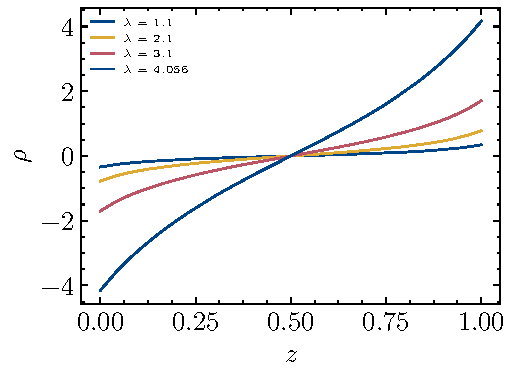
\includegraphics[width=\linewidth]{figures/neumann/vacuumPolarizationEvolution.pdf}
\end{subfigure}
\begin{subfigure}{0.5\textwidth}
    \centering
    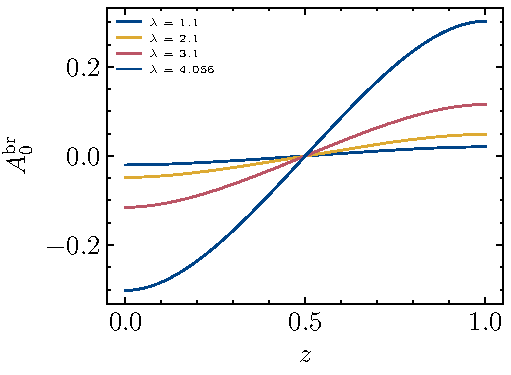
\includegraphics[width=\linewidth]{figures/neumann/A0InducedEvolution.pdf}
\end{subfigure}
\caption{The self-consistent vacuum polarizations $\rho(z)$ (left) and induced electric potentials $A_0^\text{br}(z)$ (right) of the Klein-Gordon field for Neumann boundary conditions $\partial_z \phi \rvert_{z=0,1}=0$ for selected values of $\lambda$.}
    \label{fig:vacuumPolarizatoinEvolutionNeumann}
\end{figure}

Finally, Figure \ref{fig:inducedChargeNeumann} displays the induced charge $Q_I$ (introduced in the previous section) as a function of $\lambda$ in the left panel, as well as the total electric field observed at $z=1/2$,  $\lambda + Q_I$, in the right panel. For Neumann boundary conditions, we no longer observe a 'perturbative' region where the vacuum polarization shows a clear linear increase with $\lambda$.

However, we do again observe a screening of the background electric field that prevents the total electric field $\lambda+Q_I$ to getting to the critical $\lambda_c \sim 4$ with Neumann boundary conditions.

\begin{figure}
 \begin{subfigure}{0.5\textwidth}
    \centering
    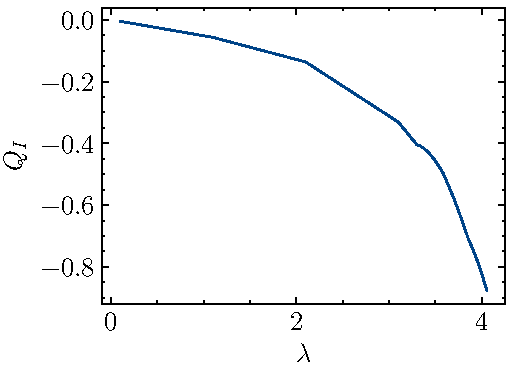
\includegraphics[width=\linewidth]{figures/neumann/inducedCharge.pdf}
 \end{subfigure}
 \begin{subfigure}{0.5\textwidth}
    \centering
    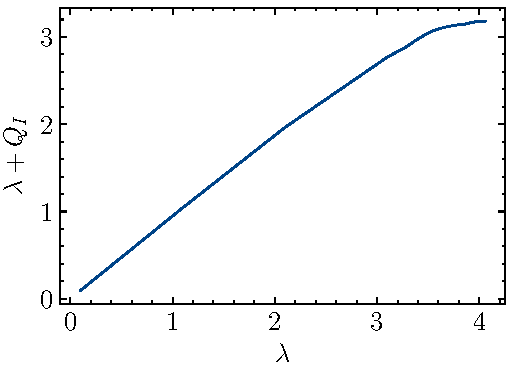
\includegraphics[width=\linewidth]{figures/neumann/electricFieldInduced.pdf}
 \end{subfigure}
\caption{The induced charge $Q_I$ in the left half-region $z\in [0, 1/2]$ (left panel) and total measured electric field at $z=1/2$, $\lambda + Q_I$ (right panel) for the Klein-Gordon field with Neumann boundary conditions as a function of the external electric field strength $\lambda$.}
    \label{fig:inducedChargeNeumann}
\end{figure}

%%%%%%%%%%%%%%%%%%%%%%%%%%%%%%%%%%%%%%%%%%%%%%%%%%%%%%%%%%%%%%%%%
\subsection{In comparison with \cite{Ambj1983}}

\cite{Ambj1983} calculates the vacuum polarization without taking into account the parallel transport with respect to the gauge covariant derivative. Moreover, in the mode decomposition of the vacuum polarization only the first mode is considered. We have shown in Figure \ref{fig:perturbative-rho-comparison} the comparison between the perturbative incorrect non-inclusion of the parallel transport (blue) and with the inclusion thereof (orange). This figure illustrates a strong difference between these two recovered quantities. The left pane of Figure \ref{fig:lowLambdaVacuumPolarization} shows the comparison between the self-consistent vacuum polarizations, as calculated by including (orange) or not including (blue) the parallel transport in the renormalization procedure. For lower values of $\lambda$ the behavior of the self-consistent vacuum polarization is identical to the perturbative approximation, and therefore it is no surprise that for these values of $\lambda$ the self-consistent vacuum polarizations also present such big differences in behavior. 

However, as $\lambda$ increases and the system diverges from the perturbative behavior, the vacuum polarization calculated using Hadamard point-splitting rapidly "catches up" to the mode sum formula vacuum polarization. This explains how the correct renormalization procedure, although much weaker at lower values of $\lambda$, is also able to screen the background electric field as it increases.

\begin{figure}
\begin{subfigure}{0.5\textwidth}
    \centering
    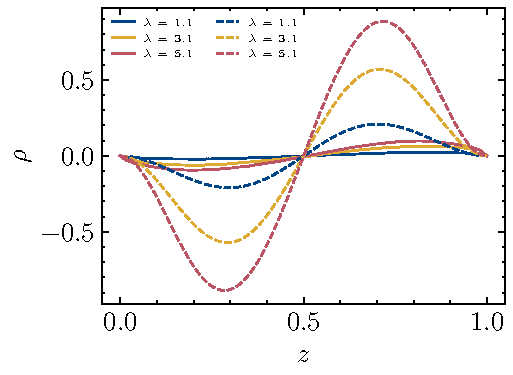
\includegraphics[width=\linewidth]{figures/dirichlet/lowLambdaVacuumPolarizationComparison.pdf}
\end{subfigure}
\begin{subfigure}{0.5\textwidth}
    \centering
    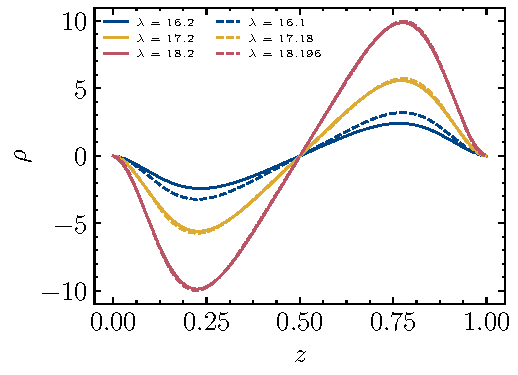
\includegraphics[width=\linewidth]{figures/dirichlet/vacuumPolarizationEvolutionComparison.pdf} 
 \end{subfigure}
 \caption{Self-consistent vacuum polarizations for low $\lambda$ (left pane) as calculated using the (wrong) mode sum formula used in \cite{Ambj1983} in blue and the (correct) Hadamard point-splitting renormalization procedure described in the previous sections in orange. In the right pane, high $\lambda$ comparison of the self-consistent vacuum polarizations for $\lambda = 16, 17, 18.4$, beyond the critical $\lambda_c$. These comparisons need to be made in different plots due to the difference in scale of 2 orders of magnitude.}
    \label{fig:lowLambdaVacuumPolarization}
\end{figure}

Figure \ref{fig:different-lambda-rho} presents the induced charged $Q_I$ defined in the previous section for both renormalization schemes. This figure shows how the effective screening of the two methods are almost identical for higher values of $\lambda$.
\begin{figure}
\begin{subfigure}{0.5\textwidth}
    \centering
    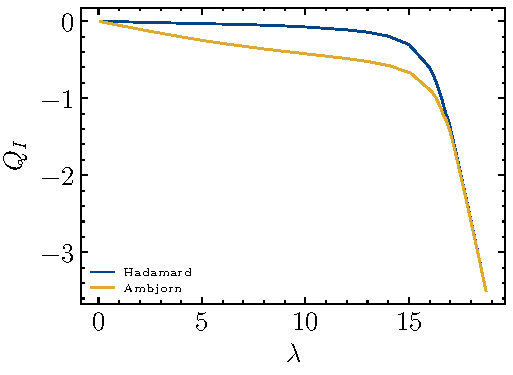
\includegraphics[width=\linewidth]{figures/dirichlet/inducedChargeComparison.pdf}
\begin{subfigure}{0.5\textwidth}
\end{subfigure}
    \centering
    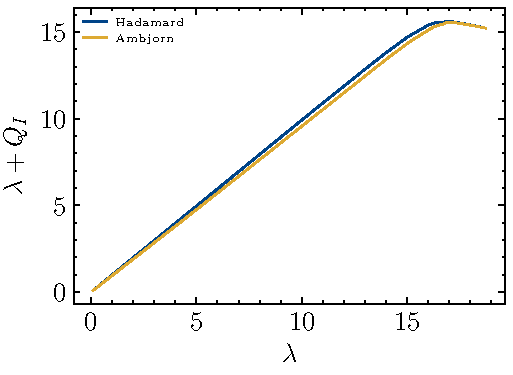
\includegraphics[width=\linewidth]{figures/dirichlet/electricFieldInducedComparison.pdf}
\end{subfigure}
\caption{Comparison of the total electric field measured at $z=1/2$ for the two renormalization procedures. In blue, the electric field corresponding to the vacuum polarization as calculated by renormalization with respect to the Hadamard parametrix. In yellow, the resulting screening due to the vacuum polarization, when calculated using the mode sum formula as was used in \cite{Ambj1983}. Notice the perturbative region for $0 <\lambda \lesssim10$. For $\lambda \gtrsim 10$, the system can no longer be approximated to the perturbative case. } 
    \label{fig:different-lambda-rho}
\end{figure}

The induced electromagnetic potential $A_0^\text{br}$, being the second integral of the vacuum polarization presents the same behavior. 
\begin{figure}
    \centering
    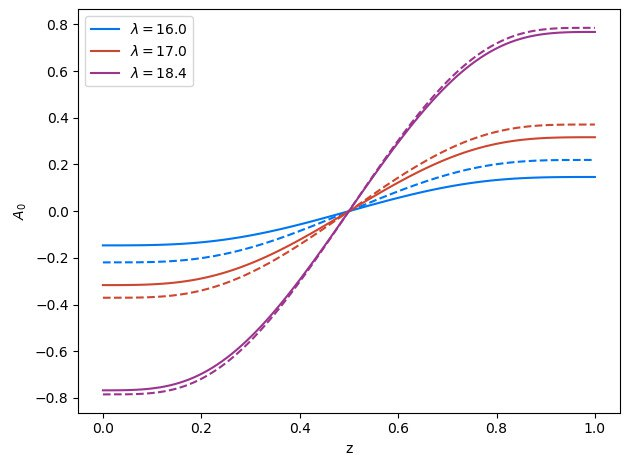
\includegraphics[width=0.5\linewidth]{figures/dirichlet/highLambdaValuesA0Induced.jpg}
    \caption{Comparison of the induced potentials $A_0^\text{br}$ using the same format as figure \ref{fig:highLambdaVacuumPolarization}.}
    \label{fig:enter-label}
\end{figure}

